\documentclass[12pt]{article}
\usepackage{titling}
\usepackage{graphicx}
\usepackage[top=1in, bottom=1.5in, left=1in, right=1in]{geometry}

\title{Designing a Hobbiest Embedded Microcontroller Laboratory}
\author{Team 12 \\ Stuart Larsen \ \ \ \ \   Troy Drabek \\ Keegan Larkin \ \ \ \ \   Adam Funkenbusch \\ Andrew Wallis }
\date{\today}

\begin{document}
\maketitle
\thispagestyle{empty}

\pagebreak


\section{Team Members}
\begin{center}
  \begin{tabular}{  l | p{8cm} | l }
    Name & Position & Email \\
    \hline
    Stuart Larsen & Project Lead & sclarsen@mtu.edu \\ 
    Troy Drabek & Expert in Microcontroller Design & tqdrabek@mtu.edu \\
    Keegan Larkin & Expert in Fabrication and Synthsis of Macro Quantum Electrodynamic Embedded Devices  & kjlarkin@mtu.edu \\
    Andrew Wallis & Resident Process Failure Mode and Effects Analysis Guru & amwallis@mtu.edu \\
    Adam Funkenbusch & Expert wire cutter & aefunken@mtu.edu \\
  \end{tabular}
\end{center}

\section{Overview and Orientation}
  The current design for the laboratory entails multiple lab benches configured to ease in the development of software systems for popular microcontroller and embedded systems. Included in the laboratory will also be a station for the fabrication of new custom embedded systems.

\subsection{Design and Goals}
The purpose of this project is to design an Embedded Microcontroller Laboratory. Due to the open endedness of the problem, we created restrains to bound the solution space into a smaller set. The following outlines our goals in designing the Embedded Microcontroller Laboratory.

\begin{enumerate}
  \item Create a lab to be used by hobbiest in the field of Embedded Microcontrollers
  \item Ease of use is number one priority, followed by cost
  \item Have a moderately wide selection of popular and available embedded microcontrollers
  \item Keep a wide supply of modules/dongles/slaves/sheids that can ease the speed of development and inspire creativity
\end{enumerate}

\subsection{Layout}

\begin{figure}[h!]
  \centering
  \fbox{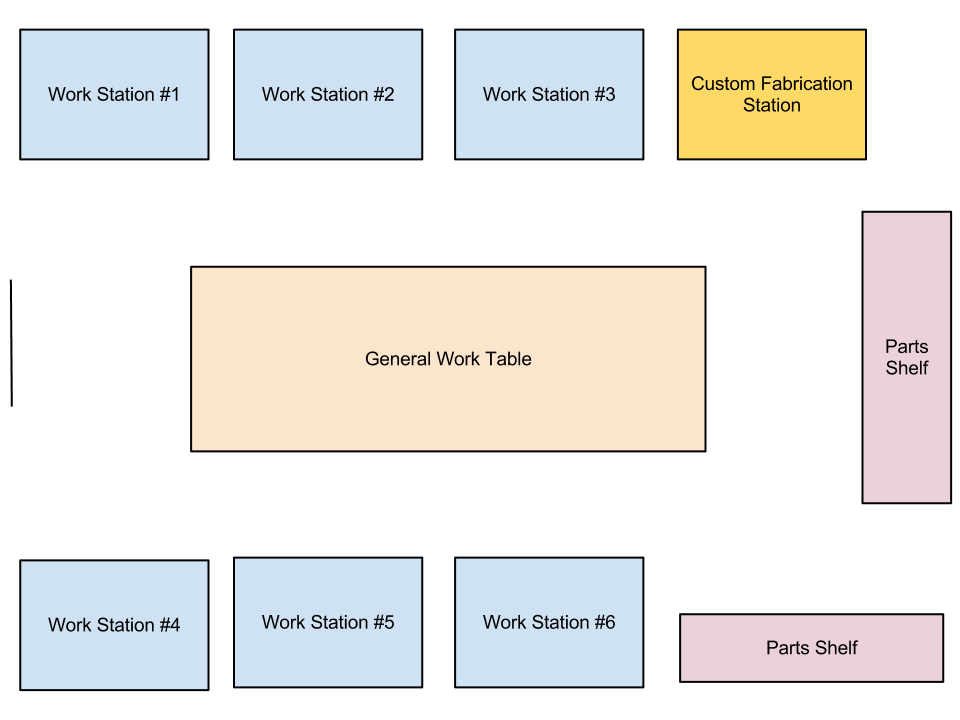
\includegraphics[scale=.4]{images/layout}}
  \label{fig:layout}
  \caption{Layout design of the laboratory}
\end{figure}
\noindent
We designed the lab with ease of use in mind. The room was designed to have room for six workstations, a custom fabrication station, a general work table, and part shelves.  \\

\noindent
Each workstation will have it's own computer preloaded with all the needed software to run the programs. The stations will also be equiped with the necessary equipment to develop and work on embedded devices, such as programmers, simple sensors, resistor/capacitor boxes, hobbiest motors and other actuators along with soldering iron/solder and breadboards. \\

\noindent
The custom fabrication station will be used in the development of custom devices for when a standard board won't work. The station will contain specialized software and equipment for fabrication that the other stations won't have.\\

\noindent
The general work table is reserved for Air Force hobbyest generals. It'll be used when more work space is required, or for holding meetings. By default the general work table shouldn't have anything except for a conference phone.

\subsection{Cost}
\noindent
Budgeting is a major concern for this project. While we don't want cost to get in the way of creativity and design, we still want the price of the lab to be as low as possible. \\

\noindent
Rough estimates are about 10k for the complete lab. 



\end{document}
